\newpage
\subsection{Messen der Slew Rate}\label{sec:3-1}
\subsubsection{Aufgabenstellung}
Mithilfe der nichtinvertierenden Verstärkerschaltung sei die Slew Rate von $A_3$ zu messen. Die Verstärkung muss $A_{GK} = 2$ betragen.


\subsubsection{Versuchsaufbau}
Zur Messung der Slew Rate wird die Schaltung aus Abbildung~\ref{fig:nichtinvertierender-verstaerker} verwendet. An $U_a$ wird das Osziloskop geschlossen. $U_1$ wurde mittels des Funktionsgenerators auf ein Rechtecksignal mit $V_{PP}=\SI{2.5}{V}$ gesetzt. Der OP-$A_3$, $R_1$ und $R_2$ sind auf dem Messverstärkerbrett (siehe Geräteliste~\ref{sec:geraeteliste})

\begin{figure}[h]
	\centering
	\begin{circuitikz}[scale=0.9, transform shape]
		% siehe PR3/latex/main-report.tex 
		\myNIA{A3}{(0,0)}{$R_1$}{$R_2$};
		\draw (A3-in) to[open, v_={$U_1$}, o-o] (A3-in |- A3-gnd) node[ground]{};
		\draw (A3-out) to[open, v^={$U_A$},o-o] (A3-out |- A3-gnd) node[ground]{};
	\end{circuitikz}
	\caption{Nichtinvertierender Verstärker}\label{fig:nichtinvertierender-verstaerker}
\end{figure}

Die Übertragungsfunktion ist ein einfacher Spannungsteiler
\begin{gather}
	A_{GK}=\frac{U_A}{U_1} = \frac{R_2+R_1}{R_1} = 1 + \frac{R_2}{R_1} \\
	A_{GK}\overset{!}{=} 2 \; \implies \; R_2=R_1
\end{gather}

Für die Messung wurde $R_1=R_2=\SI{1}{\kilo\ohm}$ gewählt.

\subsubsection{Messung}

Das Osziloskop wurde auf single Shot, mit rising Edge Trigger gestellt. Anhand
der Steigung von $U_A$ ist dann die Slew Rate abzulesen.

Aus \autoref{fig:slew-rate} werden die Werte $\Delta U = \SI{9.4}{\volt}$ und $\Delta t = \SI{20}{\mu\second}$ abgelesen.

\begin{gather}
	S_A = \frac{\Delta U}{\Delta t}\frac{\SI{9.4}{\volt}}{\SI{20}{\mu\second}} = \SI{0.47}{\volt/\mu\second}
\end{gather}

\begin{figure}
	\begin{center}
		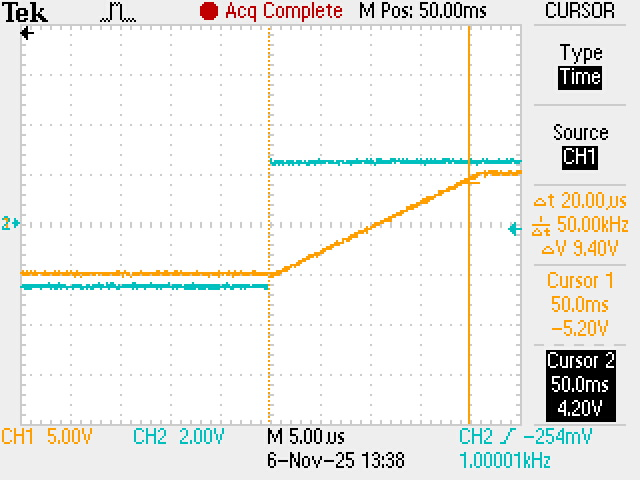
\includegraphics[width=0.65\textwidth]{images/SlewRate.JPG}
	\end{center}
	\caption{Messung der Slew Rate mit Rechteckseingangssignal}\label{fig:slew-rate}
\end{figure}

\subsubsection{Erkenntnisse}

Die Slew Rate ist mit $\SI{0.47}{\volt/\mu\second}$ sehr niedrig. Im
Skript~\cite[S.~69]{EMTPraktikum2025} steht das typische Werte zwischen
$\SI{0.6}{\volt/\mu\second}$ und $\SI{3000}{\volt/\mu\second}$ liegen. Unser OP
ist damit als langsamer Verstärker einzuordnen. Im Datenblatt des
Herstellers~\cite[S.~150, Abb.~A.3]{EMTPraktikum2025} ist für \SI{25}{\celsius}
eine Slew Rate von $\SI{0.5}{\volt/\mu\second}$ typisch. Dieser OP ist also ein
wenig langsamer als typisch. Der Operator muss auf Frequenzen beschränkt werden
($f_{\text{max}}$), bei welcher die Slew Rate mithalten kann. Ansonsten wird
das ausgangssignal verzerrt.
\[
	f_{\text{max}}=\frac{S_R}{\hat{U}2\pi}
\]
